\documentclass{article}

\usepackage[english]{babel}
\usepackage[utf8]{inputenc}
\usepackage{amsmath}
\usepackage{amsthm}
\usepackage{amssymb}
\usepackage{mathtools}
\usepackage{amsfonts}
\usepackage{subcaption}
\usepackage{graphicx}
\usepackage{wrapfig}
\usepackage{bbm}
\usepackage{dsfont}
\usepackage{listings}

% set up margin
\usepackage
[
  a4paper,
  left=3cm,
  right=3cm,
  top=3cm,
  bottom=3cm,
]
{geometry}

% set up header
\usepackage{fancyhdr}
\pagestyle{fancy}
\fancyhf{}
\lhead{6.438 Algorithms for Inference}
\chead{Problem Set 7}
\rhead{Hongzi Mao}
\cfoot{\thepage}
\rfoot{\footnotesize{\emph{Collaborated with: Hongzhou Ye, Zhiwei Ding}}}

% footer line
\renewcommand{\footrulewidth}{0.4pt}

% sans serif italic
\newcommand{\s}[1]{\textsf{\textit{#1}}}

% bold face sans serif
\newcommand{\bs}[1]{\textsf{\textbf{#1}}}

% set symbol
\usepackage[mathscr]{euscript}

% empty set
\let\emptyset\varnothing

% qed
\newcommand{\qeds}{\hfill\qedsymbol}

% math bold face
\newcommand{\bm}{\mathbf}

% argmax
\DeclareMathOperator*{\argmax}{argmax}
\DeclareMathOperator*{\argmin}{argmin}

% colorful reference
\usepackage{hyperref}
\usepackage{color}
\definecolor{darkred}{rgb}{0.7,0,0}
\definecolor{darkgreen}{rgb}{0,0.5,0}
\hypersetup{colorlinks=true,
        linkcolor=darkred,
        citecolor=darkgreen}
\urlstyle{same}

% independence symbol
\makeatletter
\newcommand*{\indep}{%
  \mathbin{%
    \mathpalette{\@indep}{}%
  }%
}
\newcommand*{\nindep}{%
  \mathbin{%                   % The final symbol is a binary math operator
    \mathpalette{\@indep}{\not}% \mathpalette helps for the adaptation
                               % of the symbol to the different math styles.
  }%
}
\newcommand*{\@indep}[2]{%
  \sbox0{$#1\perp\m@th$}%        box 0 contains \perp symbol
  \sbox2{$#1=$}%                 box 2 for the height of =
  \sbox4{$#1\vcenter{}$}%        box 4 for the height of the math axis
  \rlap{\copy0}%                 first \perp
  \dimen@=\dimexpr\ht2-\ht4-.2pt\relax
  \kern\dimen@
  {#2}
  \kern\dimen@
  \copy0 %                       second \perp
} 
\makeatother

%%%%%%%%%%%%%%%%%%%%%%%%%%%%%%%%%%%%%%%%%%%%%%%%%%%%%%%%%%%%%%%%%%%%%%%%
%%%%%%%%%%%%%%%%%%%%%%%%% Begin document here %%%%%%%%%%%%%%%%%%%%%%%%%%
%%%%%%%%%%%%%%%%%%%%%%%%%%%%%%%%%%%%%%%%%%%%%%%%%%%%%%%%%%%%%%%%%%%%%%%%
\begin{document}

\section*{Problem 7.1}
According to Hoeffding's inequality, we have for i.i.d. Bernoulli random variables $X_1, X_2, \cdots, X_M$ with $X_i \sim \text{Ber}(x + \epsilon)$,
\begin{align}
	\Pr\left[ (x + \epsilon - \eta)M \leq \sum_{i=1}^M X_i \leq (x + \epsilon + \eta)M \right] \geq 1 - 2\exp(-2\eta^2 M). \label{eq:1a_hoeffding}
\end{align}

Notice that
\begin{align*}
	\Pr(|\hat{q}(1) - p(1)| \geq t) &= \Pr\left(\left|\frac{1}{M}\sum_{i=1}^M X_i - x\right| \geq t\right) \\
	&= 1 - \Pr\left(x - t \leq \frac{1}{M}\sum_{i=1}^M X_i \leq x + t\right) \\
	&= 1 - \Pr\left(M(x - t) \leq \sum_{i=1}^M X_i \leq M(x + t)\right).
\end{align*}

Now we set $\eta = t - \epsilon$, then we have
\begin{align*}
	\Pr(|\hat{q}(1) - p(1)| \geq t) &= 1 - \Pr\left(M(x - \epsilon - \eta) \leq \sum_{i=1}^M X_i \leq M(x + \epsilon + \eta)\right) \\
	&\leq 1 - \Pr\left(M(x + \epsilon - \eta) \leq \sum_{i=1}^M X_i \leq M(x + \epsilon + \eta)\right) \;\;\; \text{(since $\epsilon > 0$)} \\
	&\leq 2e^{-2M(t-\epsilon)^2} \quad \text{(from Equation \ref{eq:1a_hoeffding})}.
\end{align*} \qeds

%
%We first check $\mathbb{P}\left(\hat{q}(1) \geq p(1) + t = x + t\right)$. Consider Chernoff bound, where for any $\eta > 0$,
%\begin{align*}
%	\mathbb{P}\left(\hat{q}(1) \geq x + t\right) &\leq 
%	e^{-\eta(x + t)}\mathbb{E}\left[\prod_{i=1}^M e^{\eta X_i}\right]\\
%	&= e^{-\eta(x + t)} \prod_{i=1}^M \mathbb{E}\left[e^{\eta X_i}\right],
%\end{align*}
%where the last equality is because $X_i$ are i.i.d. and $\mathbb{E}\left[f(x_1)f(x_2)\cdots\right] = \sum_{x_1, x_2, \cdots}[p(x_1)p(x_2)\cdots f(x_1)f(x_2)\cdots] = \sum_{x_1}[p(x_1)f(x_1)] \sum_{x_2}[p(x_2)f(x_2)] \cdots = \mathbb{E}[f(x_1)] \mathbb{E}[f(x_2)]\cdots$. Now,
%%
%\begin{align*}
%	\mathbb{P}\left(\hat{q}(1) \geq x + t\right) &\leq 
%	e^{-\eta(x + t)}
%	[(x + \epsilon) e^\eta + (1 - x -\epsilon)]^M \\
%	&= e^{-\eta(x + t)} [1 + (x + \epsilon) (e^\eta - 1)]^M \\
%	&\leq e^{-\eta(x + t)} e^{M(x + \epsilon) (e^\eta - 1)},
%\end{align*}
%where the last inequality leverages the Taylor expansion of exponential functions.

\pagebreak
%%%%%%%%%%%%%%%%%%%%%%%%%%%%%%%%%%%%%%%%%%%%%%%%%%%%%%%%%%%%%%%%%%%%%%%% 
\section*{Problem 7.2}
(a) 
%
Based on the given process of generating proposals, we know
$P_{xx'} > 0$ only when the configurations $x$ and $x'$ differ by at most one entry in $i$. Otherwise, $\mu(x')P_{x'x} = 0 = \mu(x)P_{xx'}$ trivially. Without loss of generality, suppose the differentiating entry is $i$, i.e., $x_i \neq x'_i$, and $x_j = x'_j, \forall j \neq i$.
%

Now, suppose $x_i = 0$ and $x'_i = 1$. Then we know $x_j=0, \forall j \in \partial i$ (since $x'_i = 1$ is valid) and thus
\begin{align*}
	P_{xx'} &= \Pr(\text{choose $x_i$}) \times \Pr(z = 1) \times \min(1, \lambda^{z - x_i})\\
	&= \frac{1}{|\mathscr{V}|}\times\frac{1}{2} \times \min(1, \lambda),
\end{align*}
and
\begin{align*}
	P_{x'x} &= \Pr(\text{choose $x'_i$}) \times \Pr(z = 0) \times \min(1, \lambda^{z - x'_i})\\ 
	&= \frac{1}{|\mathscr{V}|}\times \frac{1}{2} \times \min(1, \lambda^{-1}).
\end{align*}
%
Now, suppose configuration $x$ has $n$ vertices in the independent set, we have (simplifying the expression by omitting edge terms, since the configurations are all valid)
\begin{align*}
	\mu(x)P_{xx'} = \frac{1}{Z} \lambda^{n} \times \frac{1}{|\mathscr{V}|}\times\frac{1}{2} \times \min(1, \lambda),
\end{align*}
and (since $x'$ has one more vertex in the independent set)
\begin{align*}
	\mu(x')P_{x'x} = \frac{1}{Z} \lambda^{n+1} \times \frac{1}{|\mathscr{V}|}\times\frac{1}{2} \times \min(1, \lambda^{-1}).
\end{align*}

In the above expressions, if $\lambda < 1$, then $\min(1, \lambda) = \lambda$ and $\mu(x)P_{xx'} = \mu(x')P_{x'x}\propto\lambda^{n+1}$. Similarly, if $lambda > 1$,then  $\min(1, \lambda^{-1}) = \lambda^{-1}$ and $\mu(x')P_{x'x} = \mu(x)P_{xx'} \propto\lambda^{n}$.
%

Also, notice that the reverse case, $x_i = 1$ and $x'_i = 0$, is reached automatically in this check. Thus, we have $\mu(x')P_{x'x} = \mu(x)P_{xx'}$ for all valid configuration $x$ and $x'$. \qeds
\\

\noindent
(b) We have
\begin{align*}
	&P_{(0, 0), (1, 0)} = \Pr(\text{choose $x_0$})\times\Pr(z = 1)\times\min(1, \lambda^{1-0}) = \frac{1}{2}\times\frac{1}{2}\times\min(1, \lambda) = \frac{1}{4}\times\min(1, \lambda),\\
	&P_{(0, 0), (0, 1)} = \Pr(\text{choose $x_1$})\times\Pr(z = 1)\times\min(1, \lambda^{1-0}) = \frac{1}{2}\times\frac{1}{2}\times\min(1, \lambda) = \frac{1}{4}\times\min(1, \lambda),
\\
	&P_{(0, 0), (0, 0)} = 1 - P_{(0, 0), (1, 0)} - P_{(0, 0), (0, 1)} = 1 - \frac{1}{2}\min(1, \lambda),\\
	&P_{(1, 0), (0, 0)} = \Pr(\text{choose $x_0$})\times\Pr(z = 0)\times\min(1, \lambda^{0-1}) = \frac{1}{2}\times\frac{1}{2}\times\min(1, \lambda^{-1}) = \frac{1}{4}\times\min(1, \lambda^{-1}),\\
	&P_{(1, 0), (0, 1)} = 0,
\\
	&P_{(1, 0), (1, 0)} = 1 - P_{(1, 0), (0, 0)} - P_{(1, 0), (0, 1)} = 1 - \frac{1}{4}\min(1, \lambda^{-1}),\\
		&P_{(0, 1), (0, 0)} = \Pr(\text{choose $x_0$})\times\Pr(z = 0)\times\min(1, \lambda^{0-1}) = \frac{1}{2}\times\frac{1}{2}\times\min(1, \lambda^{-1}) = \frac{1}{4}\times\min(1, \lambda^{-1}),\\
	&P_{(0, 1), (1, 0)} = 0,
\\
	&P_{(0, 1), (0, 1)} = 1 - P_{(0, 1), (0, 0)} - P_{(0, 1), (1, 0)} = 1 - \frac{1}{4}\min(1, \lambda^{-1}).
\end{align*}
\\

\noindent
(c) We first observe that
\begin{align*}
	\Pr(x \neq x') &= \Pr(\rho(x, x') = 1) + \Pr(\rho(x, x') = 2) + \Pr(\rho(x, x') = 3) + \cdots \\
	&\leq \Pr(\rho(x, x') = 1) + 2 \times \Pr(\rho(x, x') = 2) + 3 \times \Pr(\rho(x, x') = 3) + \cdots \\
	&= \mathbb{E}[\rho(x, x')].
\end{align*}
%

Since $(X^t, Y^t)$ is Markov in $t$, we have 
\begin{align*}
	p(X^t, Y^t) &= p(X^t, Y^t | X^{t-1}, Y^{t-1}) \times 
				  p(X^{t-1}, Y^{t-1} | X^{t-2}, Y^{t-2}) \times
				  \cdots.
\end{align*}

Thus,
\begin{align*}
	\Pr(X^t \neq Y^t) &\leq \mathbb{E}_{X^t, Y^t}[\rho(X^t, Y^t)] \\
	&= \mathbb{E}_{X^{t-1}, Y^{t-1}}
	\big[\mathbb{E}_{X^t, Y^t | X^{t-1}, Y^{t-1}}[\rho(X^t, Y^t) | X^{t-1}, Y^{t-1}]\big] \\
	&\leq e^{-\alpha}\mathbb{E}_{X^{t-1}, Y^{t-1}}[\rho(X^{t-1}, Y^{t-1})] \\
	&= e^{-\alpha}\mathbb{E}_{X^{t-2}, Y^{t-2}}\big[\mathbb{E}_{X^{t-1}, Y^{t-1} | X^{t-2}, Y^{t-2}}[\rho(X^{t-1}, Y^{t-1}) | X^{t-2}, Y^{t-2}]\big] \\
	&\leq e^{-2\alpha}\mathbb{E}_{X^{t-2}, Y^{t-2}}[\rho(X^{t-2}, Y^{t-2})] \\
	&\;\;\;\;\cdots \\
	&\leq e^{-t\alpha} \mathbb{E}_{X^0, Y^0}[\rho(X^0, Y^0)] \\
	&\leq e^{-t\alpha} \times 2|\mathscr{V}|.
\end{align*}

This means $||\mu_{x_0}^t - \mu ||_{TV} \leq \Pr(X^t \neq Y^t) \leq 2|\mathscr{V}|e^{-t\alpha}$ holds for any $x_0$ and $t$.

Therefore, to let $2|\mathscr{V}|e^{-t\alpha} \leq \epsilon$ for a minimum $t$, we have 
\begin{align*}
	T_{\text{mix}}(\epsilon) \leq \frac{1}{\alpha}\log\frac{2|\mathscr{V}|}{\epsilon}.
\end{align*} \qeds
\\

\noindent
(d)
\begin{figure}[h!]
  \centering
  \vspace{-0.3cm}
  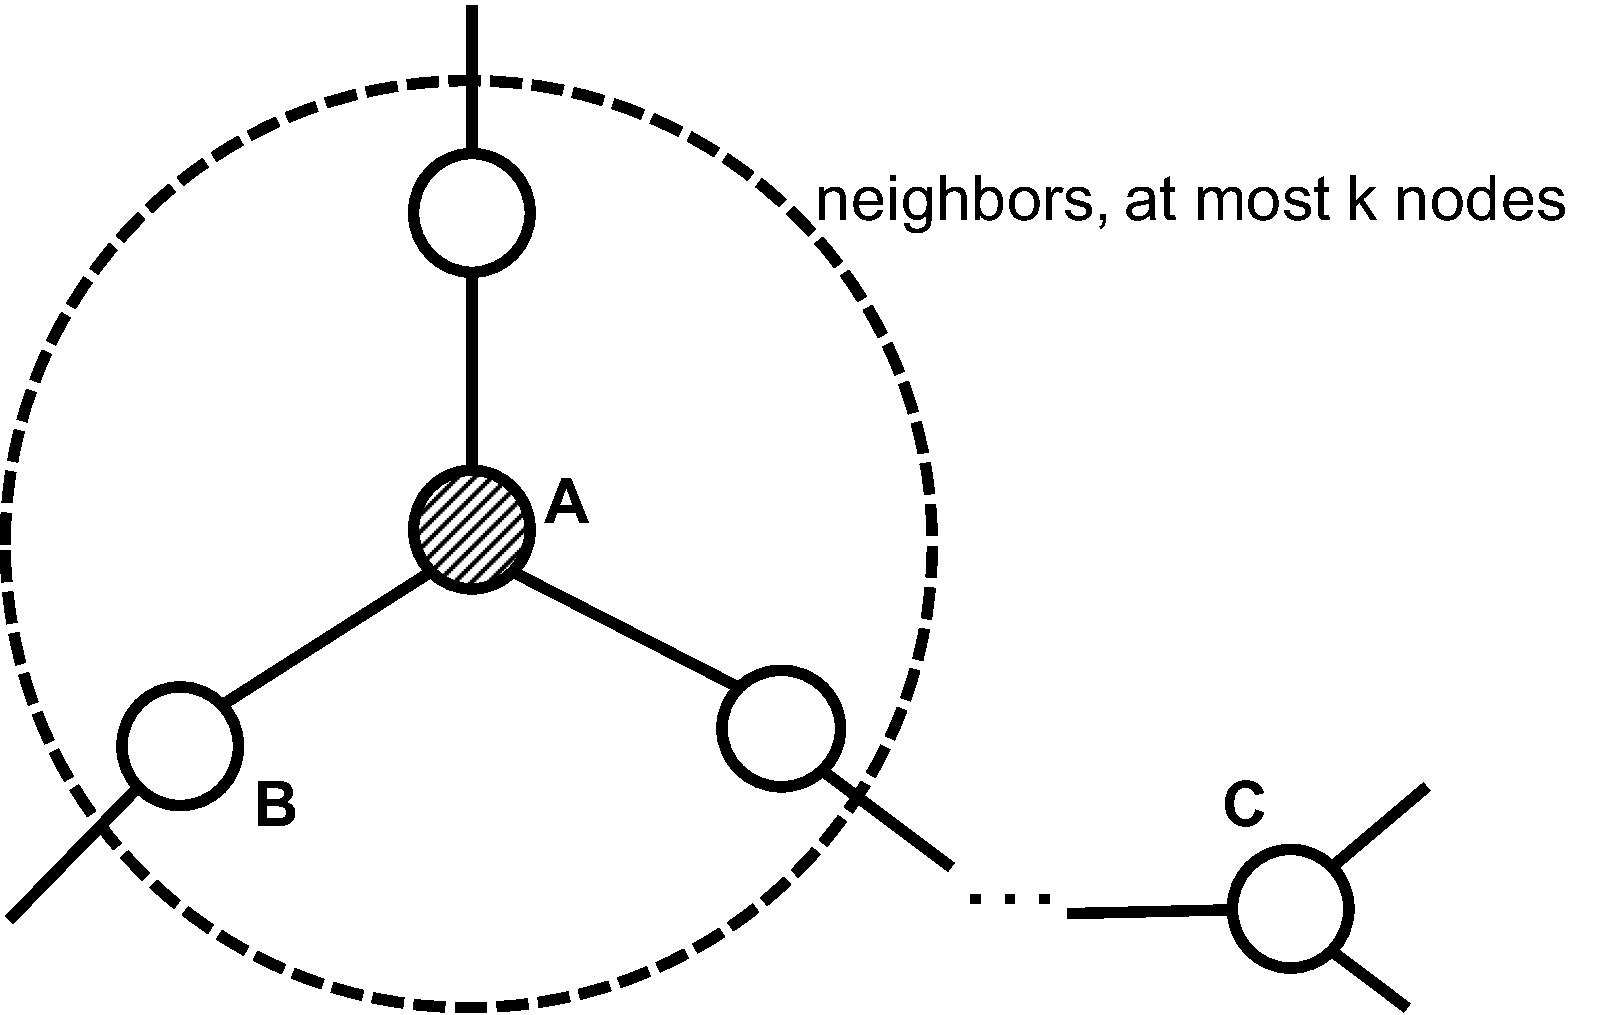
\includegraphics[width=0.5\columnwidth]{72d.pdf}
    \vspace{-0.1cm}
  \caption{Illustration graph for 7.2(d).}
  \label{f:72d}
\end{figure}
%

\noindent
Since $\rho(X^t, Y^t) = 1$, $X^t$ and $Y^t$ have to differ by a same node, otherwise,
it needs more than one flip to move from $X^t$ to $Y^t$. Let us denote this differentiating node
as $A$ in Figure~\ref{f:72d}. Without loss of generality, assume $X^t_A = 0$ and $Y^t_A = 1$. Moreover, since $Y^t_A = 1$, we know the neighbor nodes of $A$,
$X^t_{\partial A} = Y^t_{\partial A} = 0$.

Now we define the coupling $(X^{t+1}, Y^{t+1})$ to be the following procedure.
\begin{itemize}
	\item Sample the same vertex $i \in \mathscr{G}$ uniformly at random. 
	\item Then
	\begin{itemize}
		\item if the vertex $i$ is not one of the neighboring nodes of $A$
(e.g., node A or C in Figure~\ref{f:72d}),
we follow the same procedure in the problem description to stochastically flip the node.
		\item otherwise, the vertex $i$ is one of the neighboring nodes of $A$
(e.g., node B in Figure~\ref{f:72d}), we sample $U \sim \text{Unif}([0, 1])$,
and if $U < \min(1, \lambda) / 2$, we update $X^{t+1}_B = 1$ and $Y^{t+1}_B = 0$;
else $U \geq \min(1, \lambda) / 2$, we keep $X^{t+1}_B = Y^{t+1}_B = 0$.
	\end{itemize}
\end{itemize}
%

This coupling respects the update equation we considered in this problem,
because marginal $X^{t+1}$ (or $Y^{t+1}$) updates as if following the original procedure.
Specifically, if the sampled node is not in neighbors of $A$, the update rule is the
same as before. Otherwise, for $X^{t+1}_B$, the probability of flipping is $\Pr(z=1)\min(1, \lambda^{1-0}) = \min(1, \lambda) / 2$ (also, $Y^{t+1}_B$ can not be flipped because $Y^{t+1}_A=Y^{t}_A=1$).

Now, we have (in the following we use the letter $B$, $C$ to denote groups of nodes, e.g., by ``choose $B$'' we mean choose any node in neighbors of $A$)
\begin{align*}
	\mathbb{E}\big[\rho(X^{t+1}, Y^{t+1}) | X^t, Y^t \big] &= \Pr(\text{flip $X^{t+1}_B$}) \times 2 + \\
	&\;\;\;\;\; \big[\Pr(\text{choose $X^{t+1}_C$}) + \Pr(\text{choose $X^{t+1}_B$ but does not flip})\big] \times 1 \,\, + \\
	&\;\;\;\;\; \Pr(\text{choose $X^{t+1}_A$}) \times 0 \\
	&= \frac{k}{|\mathscr{V}|}\frac{\min(1, \lambda)}{2} \times 2 + (1 - \frac{k}{|\mathscr{V}|}\frac{\min(1, \lambda)}{2} - \frac{1}{|\mathscr{V}|}) \times 1 + \frac{1}{|\mathscr{V}|} \times 0 \\
	& = 1 + \frac{k}{|\mathscr{V}|}\frac{\min(1, \lambda)}{2} - \frac{1}{|\mathscr{V}|}.
\end{align*}

Notice that to satisfy $\alpha > 0$, we essentially need the above expectation to be less or equal to $1$, that is
\begin{align*}
	1 + \frac{k}{|\mathscr{V}|}\frac{\min(1, \lambda)}{2} - \frac{1}{|\mathscr{V}|} &\leq 1 \\
	\min(1, \lambda) &\leq \frac{2}{k}
\end{align*}

Thus, the condition for $\lambda$ is, $\lambda \leq 2/k$, if $k > 2$; and unconstrained if $ k \leq 2$.
\\

\noindent
(e) Equation (1) in the problem requires the expectation in the ``flipping distance'' to decay 
over time. Using similar argument in (d), suppose $\rho(X^{t-1}, Y^{t-1}) = l$ we need
\begin{align*}
	\frac{lk}{|\mathscr{V}|}\frac{\min(1, \lambda)}{2}\times(l+1) +(1 - \frac{lk}{|\mathscr{V}|}\frac{\min(1, \lambda)}{2} - \frac{l}{|\mathscr{V}|})\times l \leq l.
\end{align*}

This gives
\begin{align*}
	1 + \frac{k}{|\mathscr{V}|}\frac{\min(1, \lambda)}{2} - \frac{l}{|\mathscr{V}|} &\leq 1 \\
	\min(1, \lambda) &\leq \frac{2l}{k}.
\end{align*}

Thus, the condition in (d) automatically satisfies this inequality. \qeds
\\
\\

We also notice that the same conclusion can be shown by the path coupling
and the ``triangle inequality'' from the lecture. Specifically, we construct
a path whose adjacent nodes has distance one, that is
\begin{align*}
	Z^t_0 := X^t, \; Z^t_1, \; Z^t_2, \; \cdots, \; Z^t_{\rho(X^t, Y^t)} := Y^t.
\end{align*}

We then let each of $Z^t_i$ evolve to $Z^{t+1}_i$ with the same coupling rule in (d),
by the triangle inequality,
we have
\begin{align*}
	\rho(X^{t+1}, Y^{t+1}) \leq \sum_{i=0}^{\rho(X^t, Y^t) - 1}\rho(Z^{t+1}_i, Z^{t+1}_{i+1}).
\end{align*}

Now, notice that by the path coupling construction, we have $\rho(Z^t_i, Z^t_{i+1}) = 1$, thus
\begin{align*}
	\mathbb{E}\big[\rho(X^{t+1}, Y^{t+1}) \big| X^t, Y^t\big]
	&\leq
	\sum_{i=0}^{\rho(X^t, Y^t) - 1} \mathbb{E}\big[\rho(Z^{t+1}_i, Z^{t+1}_{i+1}) \big| X^t, Y^t\big]\\
	&\leq e^{-\alpha} \rho(X^t, Y^t) \quad \text{(from (d))}.
\end{align*}\qeds
\pagebreak

%%%%%%%%%%%%%%%%%%%%%%%%%%%%%%%%%%%%%%%%%%%%%%%%%%%%%%%%%%%%%%%%%%%%%%%% 
\section*{Problem 7.3}
(a) $\s{X}$ and $\s{Y}$ are conditionally independent given $\s{Z}$. This is because $\s{Z}$ is not in the separation set of $\s{X}$ and $\s{Y}$. We can also see this from the probability factorization. From the graphical model we have
\begin{align*}
	p(X, Y, Z, A, D) = p(X)p(Y)p(A|X,Y)(p(D|Y)p(Z|Y,D).
\end{align*}

Now we marginalize out $X, Y, Z$, we have
\begin{align*}
	p(X, Y, Z) &= \sum_{A, D}p(X, Y, Z, A, D) \\ 
	&= \sum_{A, D}p(X)p(Y)p(A|X,Y)(p(D|Y)p(Z|Y,D) \\
	&= p(X)p(Y)\sum_D(p(D|Y)p(Z|Y,D)\sum_A p(A|X,Y) \\
	&= \underbrace{p(X)}_{f(X, Z)}\underbrace{p(Y)\sum_D(p(D|Y)p(Z|Y,D)}_{g(y, Z)}.
\end{align*}
 \qeds
\\

\noindent
(b) The maximal set of $\mathscr{B}$ for $\mathscr{G}_1$ is $\{3, 4\}$.
\\

\noindent
(c) The maximal set of $\mathscr{B}$ for $\mathscr{G}_2$ is $\{5\}$.
\pagebreak

%%%%%%%%%%%%%%%%%%%%%%%%%%%%%%%%%%%%%%%%%%%%%%%%%%%%%%%%%%%%%%%%%%%%%%%% 
\section*{Problem 7.4}
(a) To show the constructed graph is a minimal I-map we need to show that it is an I-map
and that the I-map is minimal. To show it is an I-map, we note that the distribution
$p(x_1, x_2, \cdots, x_n)$ can be factorize according to the permutation order, that is
%
\begin{align}
	p(x_1, x_2, \cdots, x_3) &= \prod_{i=1}^n p(x_{\sigma_i} | x_{\sigma_1}, x_{\sigma_2}, \cdots, x_{\sigma_{i-1}}) \\
	&= \prod_{i=1}^n p(x_{\sigma_i} | x_{\pi_{\sigma_i}}), \label{eq:74a}
\end{align}
%
where Equation~\eqref{eq:74a} is because by construction
$x_{\sigma_i} \indep x_{\sigma_1, \cdots, \sigma_{i-1}}\backslash \pi_{\sigma_i} \big| \pi_{\sigma_i}$.
%
Now notice that Equation~\eqref{eq:74a} is also exactly the factorization given by the directed graphical
model (each node depends only on the parents). Therefore, the CI induced by the graph is a subset of
the CI condition induced by the distribution (since the distribution could be factorized in a
different way). That is, the constructed graph is an I-map.

To see the I-map is minimal, we prove by contradiction. Suppose we can remove an edge from the graph and
still result in an I-map, it means we could have selected a smaller set of nodes as parent for the source
node that got edge removed. This contradicts with our construction that the parent is the smallest set of
nodes that leads to the conditional independence. Therefore, the constructed I-map is minimal. \qeds


\pagebreak
%%%%%%%%%%%%%%%%%%%%%%%%%%%%%%%%%%%%%%%%%%%%%%%%%%%%%%%%%%%%%%%%%%%%%%%% 
\section*{Problem 7.5}
(a)
%
Since every node is independent of every other node, there is no edge in the corresponding maximal D-map. An undirected graphical model is shown in Figure~\ref{f:75a}.
%
\begin{figure}[h!]
  \centering
  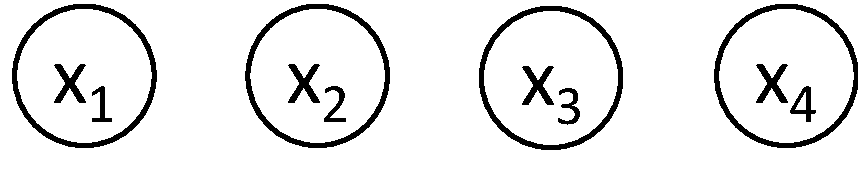
\includegraphics[width=0.3\columnwidth]{75a.pdf}
    \vspace{-0.1cm}
  \caption{Undirected graphical model for 7.5(a).}
  \label{f:75a}
\end{figure}
\\

\noindent
(b)
%
In directed graphical model, a V-structure induces conditional dependencies. Notice in the undirected graph, every non-neighboring nodes can be conditionally independent given the intermediate separating nodes. Therefore, we can not afford a V-structure in the directed graphical model. Also, directed graphical model does not have cycles. As a result, a maximal D-map is shown in Figure~\ref{f:75b} (further adding an edge in the graph either leads to a V-structure or a cycle).
%
\begin{figure}[h!]
  \centering
  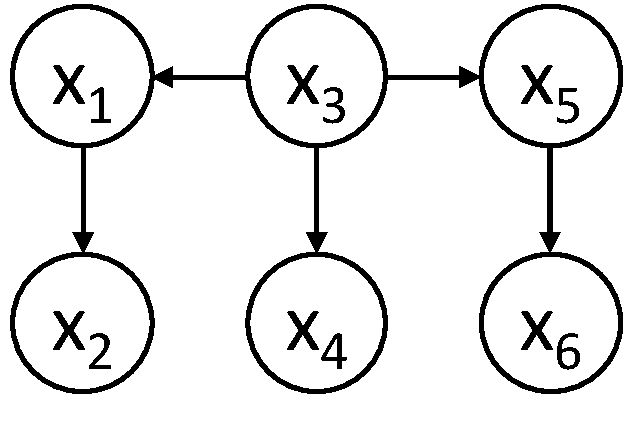
\includegraphics[width=0.225\columnwidth]{75b.pdf}
    \vspace{-0.1cm}
  \caption{Directed graphical model for 7.5(b).}
  \label{f:75b}
\end{figure}
\\

\noindent
(c)
%
It is not possible to find such a family of distribution. We show this by the following argument. First notice
that in terms of the CI condition, 
\begin{align*}
	\mathscr{I}(\mathscr{G}_{\text{I-map}}) \subseteq \mathscr{I}(p) \subseteq \mathscr{I}(\mathscr{G}_{\text{D-map}}).
\end{align*}

Thus the D-map encodes all the CI conditions encoded by the I-map.
This implies all the edges existed in the undirected D-map has to exist 
in the I-map. We prove this step by contradiction. Suppose an edge between
$x_i$, $x_j$ exists in the undirected D-map but not in the undirected I-map. 
From the I-map we have
\begin{align*}
	x_i \indep x_j \big | x_{1, 2, \cdots, n \backslash i, j}. 
\end{align*}

But this CI condition does not exist in the undirected D-map since there is
an edge between $x_i$, $x_j$. This contradicts with
$\mathscr{I}(\mathscr{G}_{\text{I-map}}) \subseteq \mathscr{I}(\mathscr{G}_{\text{D-map}})$.

Therefore the minimal I-map has to contain at least as many edges as the 
maximal D-map. That is, it is not possible to find a family of distributions
whose undirected minimal I-map has fewer edges than its undirected maximal
D-map. \qeds





\end{document}